\chapter{Estado de la Cuestión}
\label{cap:estadoDeLaCuestion}


A continuación, se abordarán diferentes aspectos referentes al proyecto y, que son de suma importancia para la comprensión de éste. Es preciso saber cómo está actualmente el campo de estudio que trata el proyecto para que al final, se pueda sacar en claro conclusiones de lo que hemos aportado y aprendido realizándolo.\\ 

En primer lugar, trataremos en líneas generales lo que es el Alzheimer y en específico, la terapia de reminiscencia y cómo ayuda a paliar esta enfermedad. Una vez ya puestos en contexto, se explicará lo que es la Inteligencia Artificial y cómo funciona exactamente, en concreto, la Inteligencia Artificial generativa de imágenes que funciona a través de redes neuronales. Lo que nos llevará al siguiente punto a tratar, qué son las redes neuronales, las diferentes variedades que existen, qué puntos positivos presenta cada una y cuál hemos elegido y por qué para implementar el modelo base que se utilizará en nuestro trabajo. \\

\section{¿Qué es el Alzheimer?}

El Alzheimer es una enfermedad que destruye lentamente la memoria y que, además, también va deteriorando los pensamientos y la conducta, hasta que poco a poco se ven afectadas las funciones más básicas. El Alzheimer es la principal causa de la demencia.\\

El cerebro envía estímulos químicos a través de las neuronas creando conexiones cerebrales, y mediante miles de millones de estas conexiones, se obtienen nuestros recuerdos, sentimientos, pensamientos y capacidades locomotoras. Aunque todavía no se sabe con certeza el motivo que causa esta enfermedad en el cerebro, se ha investigado que hay dos proteínas en el cerebro que con el tiempo se vuelven tóxicas, tau y beta-amiloide, que se acumulan hasta obstruir la conexión entre las neuronas y provocar que estas mueran, como se puede ver en \ref.  Con la destrucción de las neuronas, el cerebro se va encogiendo y con él también severamente, el hipocampo, que es una parte clave fundamental en nuestro cerebro a la hora de formar nuevos recuerdos y para el aprendizaje, lo que causa que nuestra memoria, nuestra capacidad para tomar decisiones y el habla, fallen.\\

\begin{figure}[h]
	\centering
	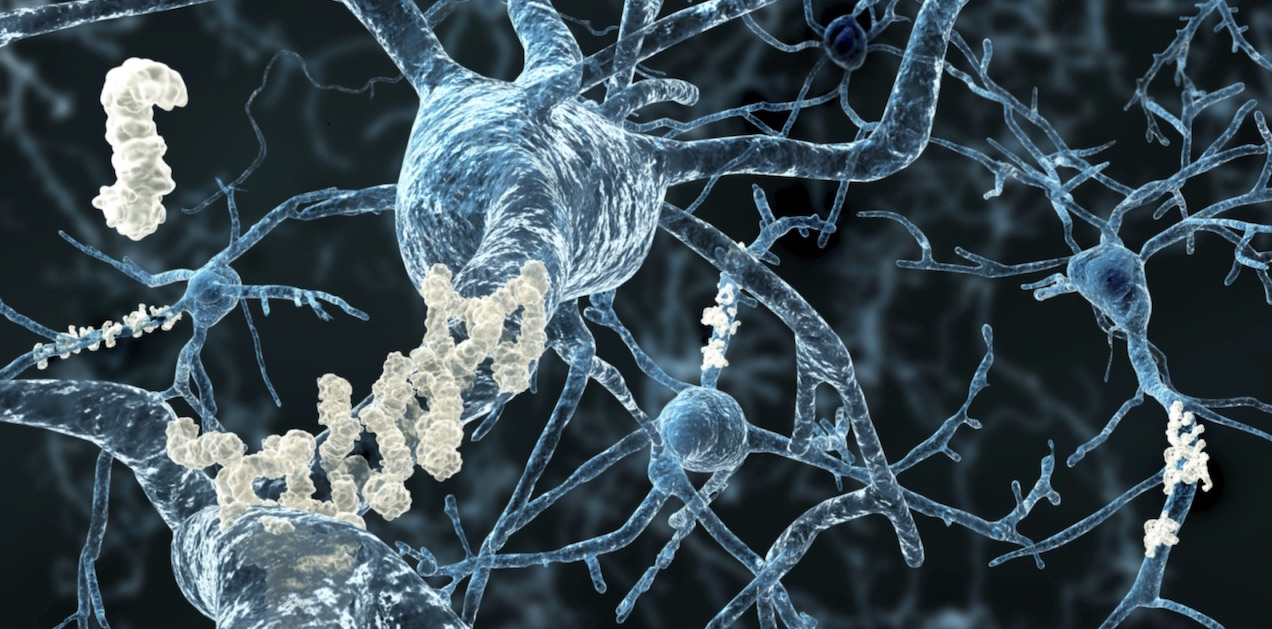
\includegraphics[width = 1 \textwidth]{Imagenes/Vectorial/proteina-tau.jpg}
	\caption{Obstrucción de neuronas por la vitamina tau}
	\label{fig:tau}
\end{figure}

\section{La terapia de reminiscencia}

Afortunadamente, existen terapias que ayudan a mejorar la calidad de vida de las personas que padecen esta enfermedad. Entre ellas la estimulación cognitiva, orientación a la realidad, ejercicio terapéutico, musicoterapia, y estimulación multisensorial, entre otras.\\
Nuestro proyecto está ligado a la terapia de reminiscencia, que es un proceso que ayuda a la persona a evocar momentos y experiencias emocionales e integrarlos en el presente, lo cual puede mejorar la autoestima y la calidad de vida.\\

En concreto, la técnica consiste en mostrar a la persona una herramienta o material visual, musical o incluso, olfativo, vinculado a su propia experiencia o hechos históricos. De esta manera se promoverá una revisión de la vida de la persona, de modo que se consiga una conexión con sus vivencias, con el fin de reconstruir un libro de vida y reforzar su identidad como persona.  Esta terapia se puede clasificar como un tipo de ensoñación que los lleva a su pasado, lo que les permite entrar en un estado de concentración con el fin de poder reforzar su memoria general, lo cual fortalece al cerebro y desarrolla sus capacidades sociales, estimula recuerdos a través de órganos sensoriales y activa su sentido de la identidad.\\

\begin{figure}[h]
	\centering
	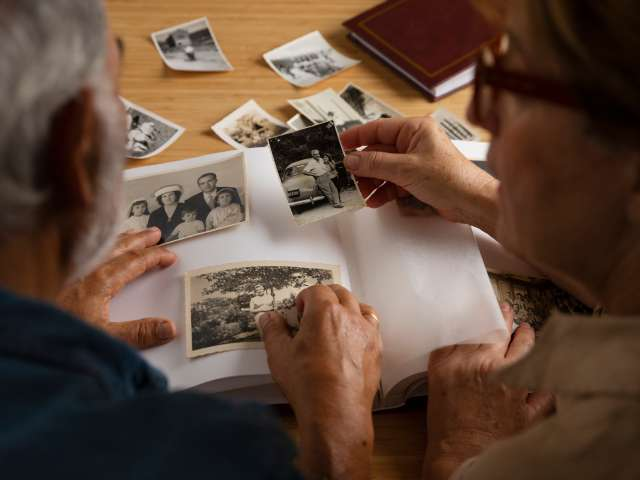
\includegraphics[width = 0.7 \textwidth]{Imagenes/Vectorial/terapiareminis.jpg}
	\caption{Terapia de reminiscencia}
	\label{fig:terapia}
\end{figure}

Algunos de los beneficios de la creación del libro de vida y la terapia ocupacional de reminiscencia, entre muchos otros, son:\\

\underline{Bienestar emocional}: Se permite que las personas puedan recordar experiencias positivas y significativas de sus vidas, lo cual puede generar sensaciones satisfactorias, de alegría y felicidad.\\

\underline{Autoconocimiento}: Cuando una persona revisa y reflexiona sobre eventos pasados y logros personales, puede obtener una comprensión de sí misma. Mediante la interacción de sus recuerdos, ayudado de la guía de cuidadores y terapeutas, puede evocar aspectos de sus valores, fortalezas y debilidades que de otra manera no serían accesibles.\\

\underline{Sentido y propósito personal}: Mediante la rememoración de escenas significativas, las personas pueden encontrar una guía emocional que permite dar sentido y dirección a sus vidas, especialmente en momentos de confusión o desorientación.\\

\underline{Reducción del estrés}: Al enfocarse en recuerdos positivos, las personas experimentan una sensación de calma, de tranquilidad y de bienestar emocional, y encuentran un espacio para escapar del estrés y tensiones del presente.\\

\underline{Favorecer las relaciones sociales}: El hecho de compartir recuerdos y experiencias con otras personas, puede fortalecer los lazos sociales y fomentar una mayor conexión con cuidadores, familia y amigos, lo cual es altamente satisfactorio para el paciente.\\

\underline{Aumentar el desarrollo del lenguaje y la persona}: Al relatar experiencias pasadas, las personas mejoran su capacidad para comunicarse de manera efectiva, así como su expresión verbal, lo cual impulsa un crecimiento personal significativo a nivel emocional e intelectual.\\

\underline{Prevenir la incapacidad}: El hecho de potenciar las habilidades lingüísticas y de mantener la mente activa, puede ayudar a preservar la función cognitiva a lo largo del tiempo. \\

Existen numerosos estudios y tesis que afirman que las capacidades cognitivas se mantienen y se consigue frenar en cierta medida el deterioro, además de reducir la ansiedad y la depresión, por lo que se hace una recomendación y un llamamiento para que se realicen estas actividades de terapia ocupacional.\\

\section{¿Qué es la Inteligencia Artificial?}

La Inteligencia Artificial es un campo de la Informática que trata la creación de herramientas, procedimientos, máquinas y computadores que simulen el proceso de inteligencia humana siendo capaces de realizar tareas como el aprendizaje, el razonamiento, la resolución de problemas, el reconocimiento de patrones, la comprensión del lenguaje natural, la percepción visual e incluso la creatividad. Este proceso se lleva a cabo utilizando principalmente el análisis de datos y las estadísticas, la ingeniería de hardware y software, aunque también abarca disciplinas como la lingüística, la neurociencia y hasta la filosofía y la psicología.\\

Ahora, existen dos tipos principales de inteligencia artificial:\\
La IA débil que se centra en tareas específicas y está diseñada para realizar funciones específicas sin poseer una inteligencia general. Y, por otro lado, la IA fuerte que busca replicar la inteligencia humana de manera más completa, con capacidad para comprender, aprender y adaptarse a una amplia variedad de tareas, con el fin de percibir su entorno y aplicando los conocimientos y datos almacenados, tener la capacidad de tomar decisiones para lograr la consecución de objetivos proporcionados.\\

Al hablar sobre inteligencia artificial, es muy importante mencionar los conceptos de aprendizaje automático (machine learning) y aprendizaje profundo (deep learning), que son subconjuntos de la inteligencia artificial que comparten la meta común de permitir a las máquinas aprender y mejorar su rendimiento en tareas específicas sin intervención humana directa.\\
El aprendizaje automático es un enfoque que abarca diferentes técnicas en las que se crean modelos de entrenamiento a partir de datos para aplicar los conocimientos adquiridos con el fin de realizar predicciones o tomar decisiones en función de nuevos datos. Es decir, se utiliza para mejorar el rendimiento de la inteligencia artificial en tareas específicas a medida que se expone a mayor cantidad de datos, que en general requiere intervención humana de forma manual.\\

Algunas categorías dentro del aprendizaje automático son:\\
- \underline{ Aprendizaje supervisado}: Un algoritmo se entrena con un conjunto de datos etiquetado, donde se le proporcionan ejemplos de entrada y la salida esperada. El modelo aprende a realizar predicciones o tomar decisiones basándose en estos ejemplos.\\

- \underline{ Aprendizaje no supervisado}: El algoritmo se enfrenta a datos no etiquetados y debe encontrar patrones o estructuras por sí mismo. Esto se utiliza comúnmente para la clasificación o agrupación de datos.\\

- \underline{ Aprendizaje por refuerzo}: El modelo aprende a través de la interacción con un entorno. Recibe recompensas o castigos según las acciones que realiza, lo que le ayuda a aprender qué comportamientos son más beneficiosos.\\

El aprendizaje profundo, a lo que respecta, es una disciplina dentro del aprendizaje automático que utiliza redes neuronales profundas con múltiples capas, que contienen datos de entrada y salida, de manera que cada capa puede aprender de la anterior a partir de los datos transformados para realizar predicciones y aprender de manera automatizada, reduciendo gran parte de la intervención humana y permitiendo aumentar el conjunto de los datos a tratar.\\

\section{Redes neuronales}

Las redes neuronales fueron creadas con el objetivo de simular el comportamiento del cerebro humano para que las máquinas pudieran ser capaces de aprender tareas computacionales de forma similar a las neuronas de nuestro sistema nervioso. La forma más básica de una neurona artificial se puede definir a través del concepto de perceptrón. El concepto de perceptrón fue visto por primera vez en 1956 por Frank Rosenblatt, psicólogo estadounidense. Un perceptrón es una unidad de red neuronal que funciona a través de un algoritmo de clasificación que realiza determinados cálculos en el que se ponderan las entradas, sumándolas y generando así una salida binaria, de manera que permite separar los datos en dos categorías. Para ello, cada entrada tiene asignada un peso que determina la relevancia de esta para su cálculo posterior en la suma ponderada, es decir, cada entrada se multiplica por su peso correspondiente para determinar su importancia relativa. La salida, además, se calcula aplicando una función de activación al resultado de la suma ponderada previamente calculada para así, dictaminar la salida final.\\

El perceptrón puede constar de una sola capa, que se compone de entrada y salida, o puede constar de múltiples capas, más conocidos como MLP (Multilayer Perceptrons). A diferencia de los perceptrones simples, los MLP constan de unas capas ocultas adicionales, componiéndose así de múltiples neuronas conectadas que se dividen típicamente en tres capas: capa de entrada, capa oculta y capa de salida. En resumidas cuentas, los perceptrones son la forma más simple de una red neuronal.\\

\begin{figure}[h]
	\centering
	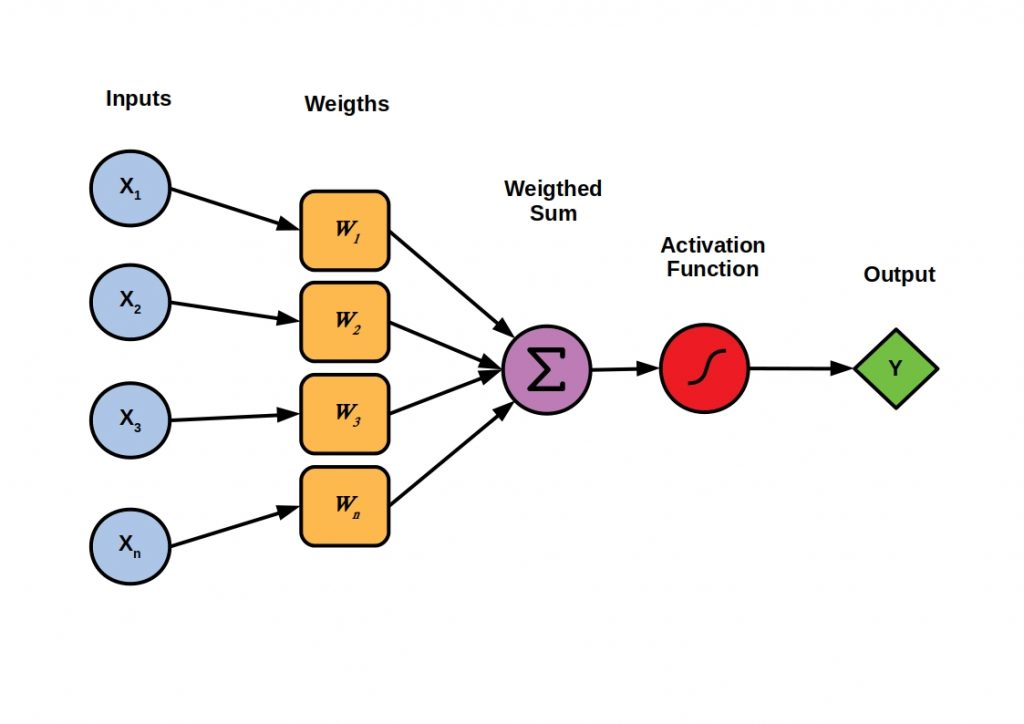
\includegraphics[width = 1 \textwidth]{Imagenes/Vectorial/Perceptrones.jpeg}
	\caption{Estructura del perceptrón}
	\label{fig:perceptron}
\end{figure}

La primera imagen generada por Inteligencia Artificial fue en 1957, por el propio creador del perceptrón, Frank Rosenblatt, quien entrenó al propio perceptrón con una serie de imágenes de rostros humanos para que éste aprendiera e identificara un patrón y reprodujera una nueva imagen. La imagen fue generada a través de una matriz de puntos de luz que aunque no se asemejara a lo que realmente era una fotografía de una persona real, hizo que este fenómeno marcará un antes y un después en el desarrollo de la Inteligencia artificial generativa.\\

\textbf{¿Qué tipos de redes neuronales existen?}\\

La variedad de redes neuronales es considerablemente grande, y cada una de ellas se han ido desarrollando y diseñando para elaborar tareas específicas. De esta manera, las diferentes redes neuronales han ido adoptando diferentes arquitecturas para tratar diferentes tipos de datos y problemas.\\
Entre ellas, mencionaremos las más relevantes hoy en día y, analizaremos el funcionamiento de cada una para tener claro cuál es la más adecuada para este modelo, haciendo una profunda comparación entre unas y otras sobre todo, nos centraremos en la red neuronal convolucional, ya que es la implementada para este trabajo.

\subsection{Redes Neuronales Feedforward (FNN)}

Son un tipo de redes multicapa, que como hemos visto, están formadas por conjuntos de neuronas agrupadas en varios niveles o capas, en los que cada neurona está conectada y recibe señales de otras neuronas pertenecientes a la capa anterior, que a su vez, se encargan de transmitir información por señales a las neuronas de la capa posterior, en dirección a la salida de la red. De esta forma, las salidas de cada capa constituyen la entrada a la capa inmediatamente posterior. En todo caso, las conexiones de la red fluyen exclusivamente en una sola y única dirección, de ahí el nombre feedforward, que traducido es hacia delante. Por norma general, la arquitectura típica que sigue una red neuronal multicapa consta de tres capas: capa de entrada, capa oculta y capa de salida. \\

Sin embargo, cabe la posibilidad de que haya más de una capa de cada tipo, y cuando se da el caso de que la red consta de más de una capa oculta, la red se califica como profunda, traducida al inglés como deep neural network. Concretamente, añadir más de una capa oculta a la red permite crear un modelo interno que reconoce patrones y proporciona un mayor rendimiento en la interpretación y estructuración de diferentes propiedades de objetos. Por ello, estas redes fueron diseñadas específicamente para resolver problemas de clasificación, regresión y por supuesto, como hemos visto, realizar reconocimiento de patrones.\\

\begin{figure}[h]
	\centering
	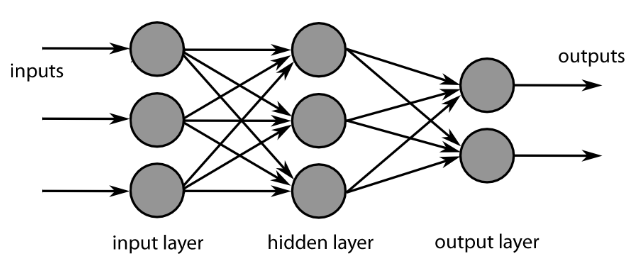
\includegraphics[width = 1 \textwidth]{Imagenes/Vectorial/feedforward.png}
	\caption{Red neuronal feedforward}
	\label{fig:feedforward}
\end{figure}



\subsection{Redes Neuronales Recurrentes (RNN)} 

Como hemos visto, las redes neuronales feedforward están habilitadas para que la información fluya en una sola dirección. Sin embargo, cuando se les proporciona una memoria, el resultado que se obtiene son las redes neuronales recurrentes, o Recurrent Neural Networks (RNN) en inglés. El origen de estas redes se popularizó en 1982 por el físico americano John Hopfield, en las que se destacan por su comportamiento dinámico y estable. \\

¿Y cómo es posible añadir memoria a las propias conexiones? Simplemente generalizando sus conexiones, es decir, alimentar a sus propias entradas o inputs con las salidas o outputs generados previamente por las conexiones anteriores provocando que el modo en el que fluyen las conexiones sea bidireccional. Es decir, incluyendo conexiones hacia atrás con las que se trabaja en una serie de pasos de tiempo, conocidos como timesteps, donde se procesan los elementos de la secuencia uno por uno, manteniendo una memoria de los estados anteriores a medida que avanzan en la secuencia.\\

El entrenamiento de redes neuronales de estas características se realiza contando con diferentes algoritmos y técnicas, la más básica y conocida en este tipo de red neuronal es el algoritmo de propagación de errores (back-propagation en inglés) formalizado en 1986 por Rumelhart, Hinton y Williams. Este método, en concreto, consiste en aplicar un patrón a la primera capa de la red, el cual se va propagando hacia las capas superiores con el objetivo de generar una salida que se pueda comparar con la salida deseada y así poder calcular el error para cada neurona de la salida obtenida en función de los diferentes parámetros de la red. En otras palabras, cómo varía el error en relación con la variación de los parámetros de la red neuronal. Si a este fenómeno le sumamos la variable del tiempo, se obtiene la técnica de retropropagación a través del tiempo (backpropagation through time, BPTT), en la que después de analizarse la secuencia completa, calcular el error y cambiar los parámetros para minimizar el mismo, se propaga el error a través del tiempo desde la última capa hasta la superior en cada paso de tiempo con el fin de que la red aprenda de las secuencias y mejore su predicción futura. 
Este método combinado con la técnica del gradiente descendiente encargada de la optimización del error buscando los parámetros adecuados para poder reducirlo al mínimo es el modo de aprendizaje supervisado más popular que existe.  Aunque, como hemos visto anteriormente, no es el único, ya que coexiste con técnicas de entrenamiento como el aprendizaje no supervisado y el aprendizaje por refuerzo. \\

Así que, podemos concluir en que las redes neuronales son idóneas para tareas de modelado de datos secuenciales y con dependencias temporales, como lo pueden ser el procesamiento de lenguaje natural, la generación de texto o la traducción automática, entre muchas otras.
\begin{figure}[h]
	\centering
	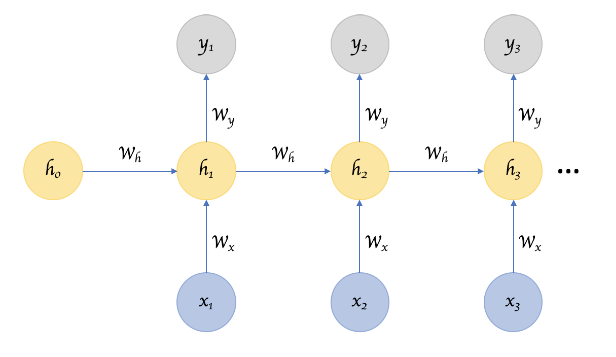
\includegraphics[width = 1 \textwidth]{Imagenes/Vectorial/recurrente.png}
	\caption{Red neuronal recurrente}
	\label{fig:rnn}
\end{figure}


\subsection{Redes Neuronales LSTM} 

Las redes neuronales Long Short-Term Memory surgen a partir de las redes neuronales recurrentes cuyo principal objetivo y propósito es ratificar el problema del desvanecimiento del gradiente. \\

En primer lugar y para entender en qué consiste este problema, es necesario saber qué es exactamente un gradiente y a qué nos referimos cuando hablamos del desvanecimiento del mismo. Un gradiente es una medida que determina la variación de una función con respecto al cambio que se produce en sus variables, ya sea en términos de optimización, rapidez o maximización de la función objetivo. \\

Matemáticamente, se puede entender como un vector multivariable cuyas variables son las derivadas parciales de dicha función. Se puede ver en el ejemplo de la figura. Geométricamente hablando, el gradiente indica la dirección en la que la función crece a mayor velocidad y, de esta manera, podemos concluir que el uso de los gradientes se hace con el fin de ajustar los parámetros para reducir al mínimo la diferencia entre los valores obtenidos y los deseados. Un claro ejemplo de ello son los modelos de predicción, en los que se busca reducir dichas predicciones con los valores reales. \\

Ahora bien, cuando hablamos del desvanecimiento del gradiente nos referimos al fenómeno que ocurre en la propagación hacia atrás, cuando a medida que se va produciendo la propagación en capas cada vez más profundas, el gradiente va disminuyendo hasta llegar a ser tan pequeño que las capas superiores sean incapaces de aprender de manera efectiva. Este tipo de problema es común en redes conformadas por una gran cantidad de capas, dado que se disminuye exponencialmente a medida que va recorriendo cada capa hasta impedir que los pesos se actualicen de manera correcta y que puedan tener un aprendizaje lo suficientemente eficiente para ser capaces de resolver patrones complejos.
La solución a este problema se abordó introduciendo nuevos componentes a la red que ayudan y controlan el flujo de información de la red, consiguiendo aumentar la memoria del conjunto de la red al almacenar la información durante periodos más largos de tiempo. Los componentes principales son los siguientes:
Memory cells o celdas de memoria: contienen la información relevante  y actualizada a lo largo del tiempo.\\ 

\underline{Input gates o puertas de entrad}a: son las encargadas de controlar la cantidad de información que entra a las celdas de memoria.\\

\underline{Forget gates o puertas de olvido}: seleccionan la información que debe ser eliminada de la celda, al no ser de utilidad.\\

\underline{Output gates o puertas de salida}: su tarea radica en seleccionar la información de la celda que va a pasar a la siguiente capa de la red, basándose en el estado oculto actual.\\

Para entender cómo funcionan y se relacionan estos componentes en la estructura de la red, lo veremos con un ejemplo hipotético en el que la celda de memoria representa una caja fuerte y las diferentes puertas son componentes de una cinta transportadora. \\

La caja fuerte contiene información valiosa que se transporta en la cinta, el la puerta de entrada actúa como una máquina que trabaja en la cinta que se encarga de introducir nueva información a la caja fuerte y regular la información contenida en esta; la puerta de olvido actúa como una máquina que descarta fragmentos de información contenidas en la caja fuerte; y por último, el componente que representa la puerta de salida, se encarga de elegir si la información contenida en la caja fuerte es apta para salir de la cinta transportadora. \\

De este modo, se consigue erradicar el problema del desvanecimiento del gradiente y se consigue procesar grandes secuencias de datos durante largos periodos de tiempo. Es especialmente útil en tareas que requieren capturar grandes dependencias de datos temporales, ejemplo de ello son el procesado y/o reconocimiento de lenguaje natural, en la traducción automática y en la generación de texto.\\

\begin{figure}[h]
	\centering
	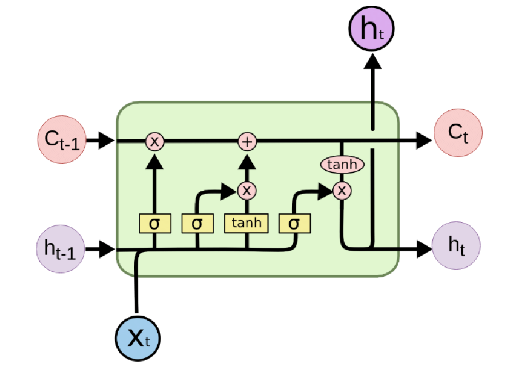
\includegraphics[width = 1 \textwidth]{Imagenes/Vectorial/lstm.png}
	\caption{Red neuronal Long Short Term Memory}
	\label{fig:lstm}
\end{figure}



\subsection{Redes Neuronales Convolutivas (CNN)}

Las redes neuronales convolucionales se introdujeron por primera vez en la década de los 50 por David Hubel y Torsten Wiesel cuando experimentaron con las neuronas biológicas, lo que le sirvió de inspiración a Kunihiko Fukushima en la década de los 80 para desarrollar el Neocognitron, una red neuronal que se conoce como la primera CNN. Este concepto fue cobrando forma con el paso de los años y el modelo tal y como lo conocemos hoy en día, fue obra de Yann LeCun en 1998 al introducir el aprendizaje a través de la técnica de backforwarding.	\\

Las redes neuronales convolutivas están formadas por una secuencia de capas que podemos clasificar en tres tipos: capas convolutivas, capas de pooling y capas completamente conectadas.\\ 

\underline{Capas convolutivas}: suponen la capa principal de la red, y el papel que desempeña en el procesamiento de imágenes, es realizar la gran parte de los cálculos que se necesitan para extraer características de las imágenes. Para ello, hace falta la intervención de tres elementos principales: datos de entrada, un filtro y un mapa de características. 

Los datos de entrada son el elemento que se trata de analizar, por ejemplo, en el caso de una imagen de color que estuviera compuesta por una matriz de píxeles en 3D, las dimensiones serían la altura, la anchura y la profundidad de la misma. 

Por otro lado, el filtro o kernel, se trata de un detector de características, que va pasando por cada área de la imagen para identificar diferentes características, este proceso se denomina convolución. 

El siguiente paso es representar mediante una matriz bidimensional de pesos, que al aplicarse en cada área calcula un producto escalar a partir de los píxeles de los datos de entrada y del filtro. El producto escalar se utiliza como input en la matriz de salida para que el filtro sea capaz de repetir el proceso por toda la imágen. La finalidad del filtro es ser capaz de distinguir diferentes patrones, como lo pueden ser texturas, bordes o figuras. 

Finalmente, la suma de los diferentes productos escalares y el o los filtros utilizados, da como resultado final lo que se conoce como mapa de características. 

Después de cada capa de convolución, se aplica una función de activación no lineal al mapa de características, a través de la ReLU (Rectified Linear Unit). El fin de esta función es introducir no linealidad a la red, lo que le permite mejorar la complejidad entre las diferentes características. \\

\underline{Capa de agrupación o pooling}: son capas dedicadas a reducir la dimensión del mapa a través de la disminución del número de parámetros de entrada.

Comúnmente, se utilizan dos técnicas conocidas como max pooling y average pooling. Max pooling consiste en seleccionar el pixel con mayor valor a medida que el filtro recorre la imagen para enviar el máximo a la matriz de salida, en cambio, average pooling lo que busca es calcular el valor medio del campo. El inconveniente que presenta esta capa es la gran pérdida de información que existe, sin embargo, presenta una gran ventaja a la hora de reducir la complejidad computacional y concentrarse en las características más importantes, lo que claramente, mejora el rendimiento del modelo y evita el riesgo de que se produzca un sobreajuste.\\

\underline{Capa totalmente conectada}: en las últimas capas de la red los nodos están conectados con los de la capa anterior para producir la salida final incorporando las características extraídas y aprendidas de los procesos realizados en las capas anteriores. Las capas totalmente conectadas se preocupan de realizar las funciones de clasificación de la imagen y de regresión para producir el resultado deseado. \\

Las principales funciones y tareas que abarcan las redes neuronales convolucionales son el reconocimiento de imágenes identificando y detectando objetos, personas o animales; análisis de imágenes para diferentes propósitos, por ejemplo, médicos; reconocimiento facial; segmentación semántica; y por supuesto, generación de imágenes.\\

\begin{figure}[h]
	\centering
	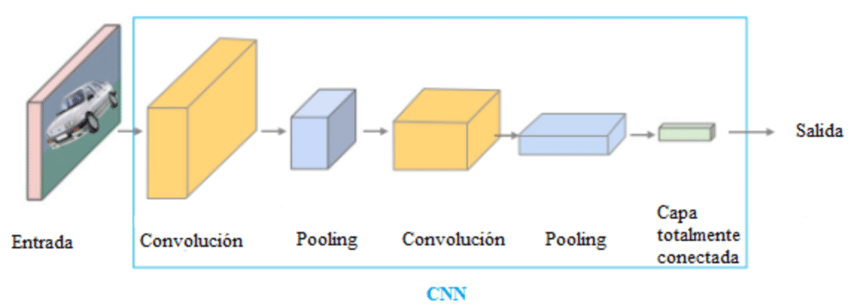
\includegraphics[width = 1 \textwidth]{Imagenes/Vectorial/cnn.png}
	\caption{Red neuronal convolucional}
	\label{fig:cnn}
\end{figure}

\subsection{Redes Generativas Adversarias (GAN)}

Las redes GAN, del inglés, Generative Adversarial Networks son un tipo de redes neuronales profundas revolucionarias, que son relativamente novedosas, ya que surgieron en el año 2014 por primera vez por Ian Goodfellow y sus compañeros en la Universidad de Montréal. \\

El funcionamiento de este tipo de redes involucra a dos redes neuronales diferentes, en las que cada una se encarga de realizar una tarea específica y “competir” contra la otra, para así, cada vez ir mejorando más los resultados obtenidos. \\

La primera red neuronal de este sistema se conoce como “Generador” y se encarga de producir y crear datos totalmente nuevos basándose en los datos aportados en el entrenamiento de la red. Se le asigna como entrada un vector de ruido y es responsable de crear datos que se asimilen a los datos originales. El entrenamiento del Generador es constante y siempre busca mejorar los resultados a medida que los va produciendo para alcanzar el máximo realismo posible. \\

La segunda red neuronal de la que se compone este sistema es el “Discriminador”, se dedica a analizar los resultados producidos por el Generador e identificar si son los reales o los creados por la red. A medida que va avanzando su entrenamiento, la capacidad del discriminador en distinguir entre un resultado real o falso dada una cierta entrada va mejorando cada vez más, haciendo que su predicción sea más certera. 
Un clásico ejemplo llevado a la vida real de esto puede ser el caso de un falsificador de billetes y un detective, en el que el primero tiene como muestra cierta cantidad de billetes e intenta replicarlos para que más adelante el segundo agente intente detectar la copia del original. A medida que pasa el tiempo, cada uno de los dos individuos van mejorando en su tarea llegando a un nivel de equilibrio. \\

Matemáticamente, el discriminador tiene que generar una salida, expresada como D(x), basándose en la probabilidad de que la entrada sea sintética o real, suponiendo que en cuanto más cercana a 1 sea, la entrada es original. Y por el contrario y dada una muestra aleatoria z en función de cierta distribución de probabilidad, el generador tiene que producir una muestra, expresada como G(z), que el discriminador tiene que clasificar como cercana a 0, produciendo una salida del tipo D(G(z)) en la que el generador tiene que intentar que su probabilidad se aproxime a 1, justo al contrario que el discriminador. Suponiendo que entre todas las muestras del modelo, una mitad son auténticas y la otra mitad son falsas, se tiene que alcanzar el conocido como equilibrio de Nash en el que las muestras del modelo son igual a los datos y en las que la probabilidad del discriminador es D(x) 0,5 para todo x. \\

Por último, cabe destacar que para el entrenamiento de este tipo de red se utilizan los métodos del gradiente descendente y backpropagation, vistos en redes neuronales anteriores. \\

Este tipo de redes son ideales para tareas que requieren creación de datos realistas y artísticos, como lo pueden ser la generación de imágenes, de música o incluso, síntesis de voz. 

\begin{figure}[h]
	\centering
	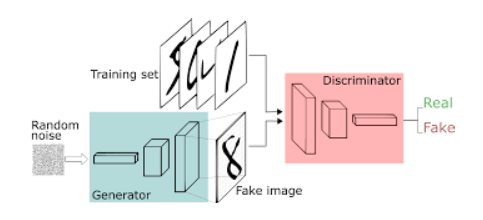
\includegraphics[width = 1 \textwidth]{Imagenes/Vectorial/gan.png}
	\caption{Red neuronal generativa antagónica}
	\label{fig:gan}
\end{figure}


\subsection{Redes Neuronales Transformer}

Las redes neuronales Transformer son las más actuales tratadas en este trabajo, surgieron en 2017 a través del artículo “Attention is all you need” elaborado por Vaswani et al.. El artículo trata una mejora de las redes recurrentes y convolucionales conocidas introduciendo un mecanismo basado sólidamente en la atención, es decir, realizar paralelismo entre las diferentes tareas que realiza la red. Para ello, se parte de una entrada mediante embedding y se hace uso de dos componentes: codificador y decodificador. \\

\underline{Embedding}: es el primer bloque por el que está compuesto la red neuronal, su función es primordial para el manejo de los datos, ya que transforma el texto de entrada en unos determinados vectores o tokens, los cuales son la representación numérica del valor inicial. \\

\underline{Codificador o encoder}:  después del embedding de la entrada, el siguiente bloque es el codificador posicional cuya tarea es indicar a la red el orden de los diferentes elementos del vector, es decir, de las palabras en el texto. Esta función es esencial ya que la secuencia se procesa en paralelo, y del contrario, no se podrían concretar las posiciones de cada uno.\\

A continuación, se encuentran conectados en secuencia los codificadores. Cada codificador se compone de 4 elementos: el bloque residual, una red neuronal, otro bloque residual, y por último, un bloque atencional siendo el más importante de todos al encargarse de determinar la relevancia de cada uno de los tokens para la frase junto a su asociación. Los restantes elementos se encargan de normalizar la entrada y la salida para poder seguir entrenando la red de forma productiva. \\

\underline{Decodificador o decoder}: cada codificador está conectado a un decodificador, que cumplen una composición similar, sino igual,  a  la explicada en los codificadores, es decir, cuatro elementos: dos bloques residuales, una red neuronal y un bloque atencional. A los que se le añaden dos elementos más en la estructura: un tercer bloque residual y un bloque atencional con enmascaramiento. \\

Sin embargo, el funcionamiento difiere al de la estructura anterior. Se comienza con el bloque atencional con enmascaramiento que codifica las relaciones entre elementos atendiendo únicamente a palabras actuales y pasadas. Por otro lado, el bloque atencional del decodificador se conecta con el del codificador para establecer el orden de prioridad al que se debe prestar atención en la secuencia, sus valores son probabilidades entre 0 y 1 siendo el valor más alto el seleccionado. Por último, el comportamiento de los demás bloques cumplen la mismas funciones que en el codificador, incluyendo entre ellos, los bloques residuales, el bloque de codificación posicional y la salida en función del embedding.  \\

Por lo tanto, podemos afirmar que estas redes neuronales aprenden contexto y significado mediante el seguimiento de relaciones en datos secuenciales. Todo tipo de organizaciones utilizan estos modelos para conversión de secuencias, incluidas las de reconocimiento de voz y la traducción automática. Esta red neuronal procesa secuencias largas con cálculo paralelo, con el objetivo de reducir significativamente el tiempo de entrenamiento y de procesamiento.
A raíz de este modelo, surgen técnicas innovadoras como el aprendizaje por transferencia y la generación aumentada de recuperación (RAG). El objetivo principal es entrenar inicialmente los modelos de conjuntos de datos amplios y después refinarlos de manera precisa, utilizando conjuntos de datos más específicos. De este modo, se maximiza su utilidad y relevancia dentro de cualquier contexto.\\

\begin{figure}[h]
	\centering
	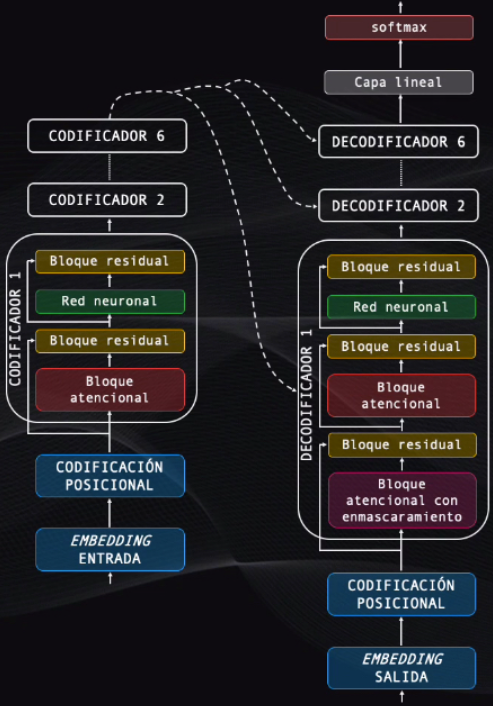
\includegraphics[width = 0.7 \textwidth]{Imagenes/Vectorial/transformer.png}
	\caption{Red neuronal Transformer}
	\label{fig:transformer}
\end{figure}

Estos suponen sólo algunos ejemplos de los tipos de redes neuronales más comunes y ampliamente utilizadas. Cada tipo tiene sus propias características, fortalezas y debilidades, y es importante elegir el tipo adecuado según el problema específico que se esté abordando y el tipo de datos disponibles.\\

 \section{Stable Diffusion}

Como hemos visto, hay diferentes redes neuronales destinadas a la generación tanto de texto como de imágenes. En el caso de Stable Diffusion, el modelo de IA utilizado en nuestro proyecto, funciona con un modelo de difusión latente basado en CNNs y en Transformers. Ya visto el comportamiento y funcionamiento de ambas redes neuronales en apartados anteriores, analizaremos más en profundidad de qué manera se integran y complementan en el modelo que utilizaremos más adelante.\\


Stable Diffusion es un modelo de Inteligencia Artificial generativa cuya principal función es transformar el texto a imagen, aunque también presenta otras funciones asombrosas como la transformación de imagen a imagen o incluso lo más novedoso hasta el momento, transformaciones de texto a vídeo. Las empresas desarrolladoras hicieron una colaboración conjunta entre CompVis LMU, Runway y Stability AI y el lanzamiento finalmente se produjo a mediados de 2022, es decir, esta poderosa herramienta relativamente nueva y los avances tecnológicos que ha alcanzado hasta la fecha son impresionantes. \\


\subsection{Funcionamiento interno de Stable Diffusion}

En principio, Stable Diffusion cuenta con un entrenamiento de más de 5 millones de imágenes proporcionado por el dataset Laion-5B que permite contar con una gran variedad de opciones de creación de imágenes, desde objetos, animales, paisajes y lugares, personas e incluso celebridades mundialmente conocidas con una calidad notable.\\ 

Comencemos entendiendo el funcionamiento del modelo de difusión latente, y para facilitar su explicación y comprensión,  lo diseccionaremos en dos partes: difusión y el espacio latente. El proceso de difusión que sigue la generación de una imagen es, en primer lugar y partiendo de las millones de imágenes del dataset mencionadas, se procede a añadir ruido gaussiano gradualmente a través de una serie de pasos hasta que las fotografías pierden todo valor y terminan siendo irreconocibles. Se podría decir que se comporta como una cadena de Markov, al ser el ruido gaussiano una variable aleatoria y al depender cada paso exclusivamente de su anterior. Este primer método se conoce como difusión directa hacia delante o forward diffusion.\\

\begin{figure}[h]
	\centering
	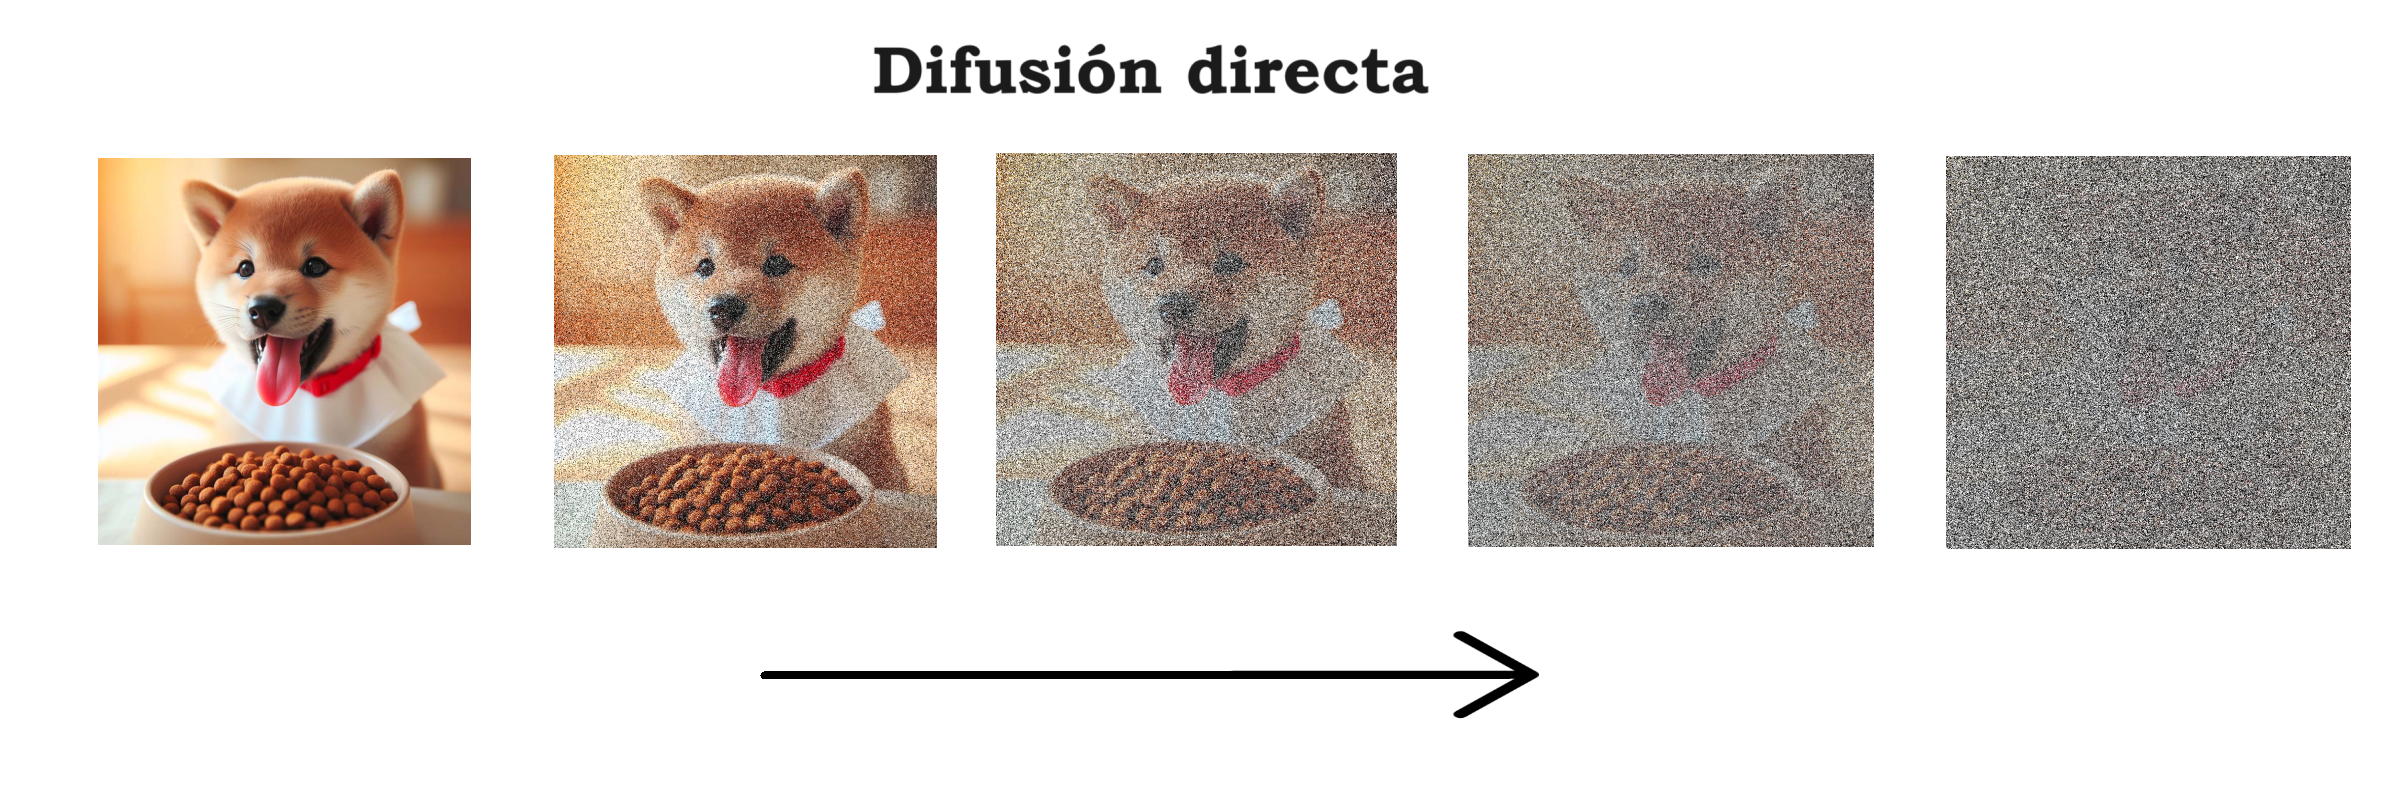
\includegraphics[width = 1 \textwidth]{Imagenes/Vectorial/difusiondirecta.png}
	\caption{difusión directa de una imagen de un cachorro de Shiba Inu comiendo}
	\label{fig:difusiondirecta}
\end{figure}

Así mismo, cuando se procesa una petición dado un prompt, se parte de una imagen únicamente hecha de ruido aleatorio, es decir, un imagen sin nada relevante ni identificable en ella. Partiendo de esta imagen llena de ruido, se intenta revertir lo hecho anteriormente para volver a la imagen original quitando el ruido gradualmente. El ruido es aleatorio, y su aleatoriedad depende de un parámetro llamado seed o semilla que asocia el ruido generado con un número aleatorio. Por lo tanto, si se repite la semilla se volverá a generar exactamente el mismo ruido y tendríamos como resultado una réplica de una imagen ya generada con esa misma semilla. Este proceso se conoce como difusión inversa y su objetivo principal es que el modelo aprenda a eliminar el ruido completamente. \\

\begin{figure}[h]
	\centering
	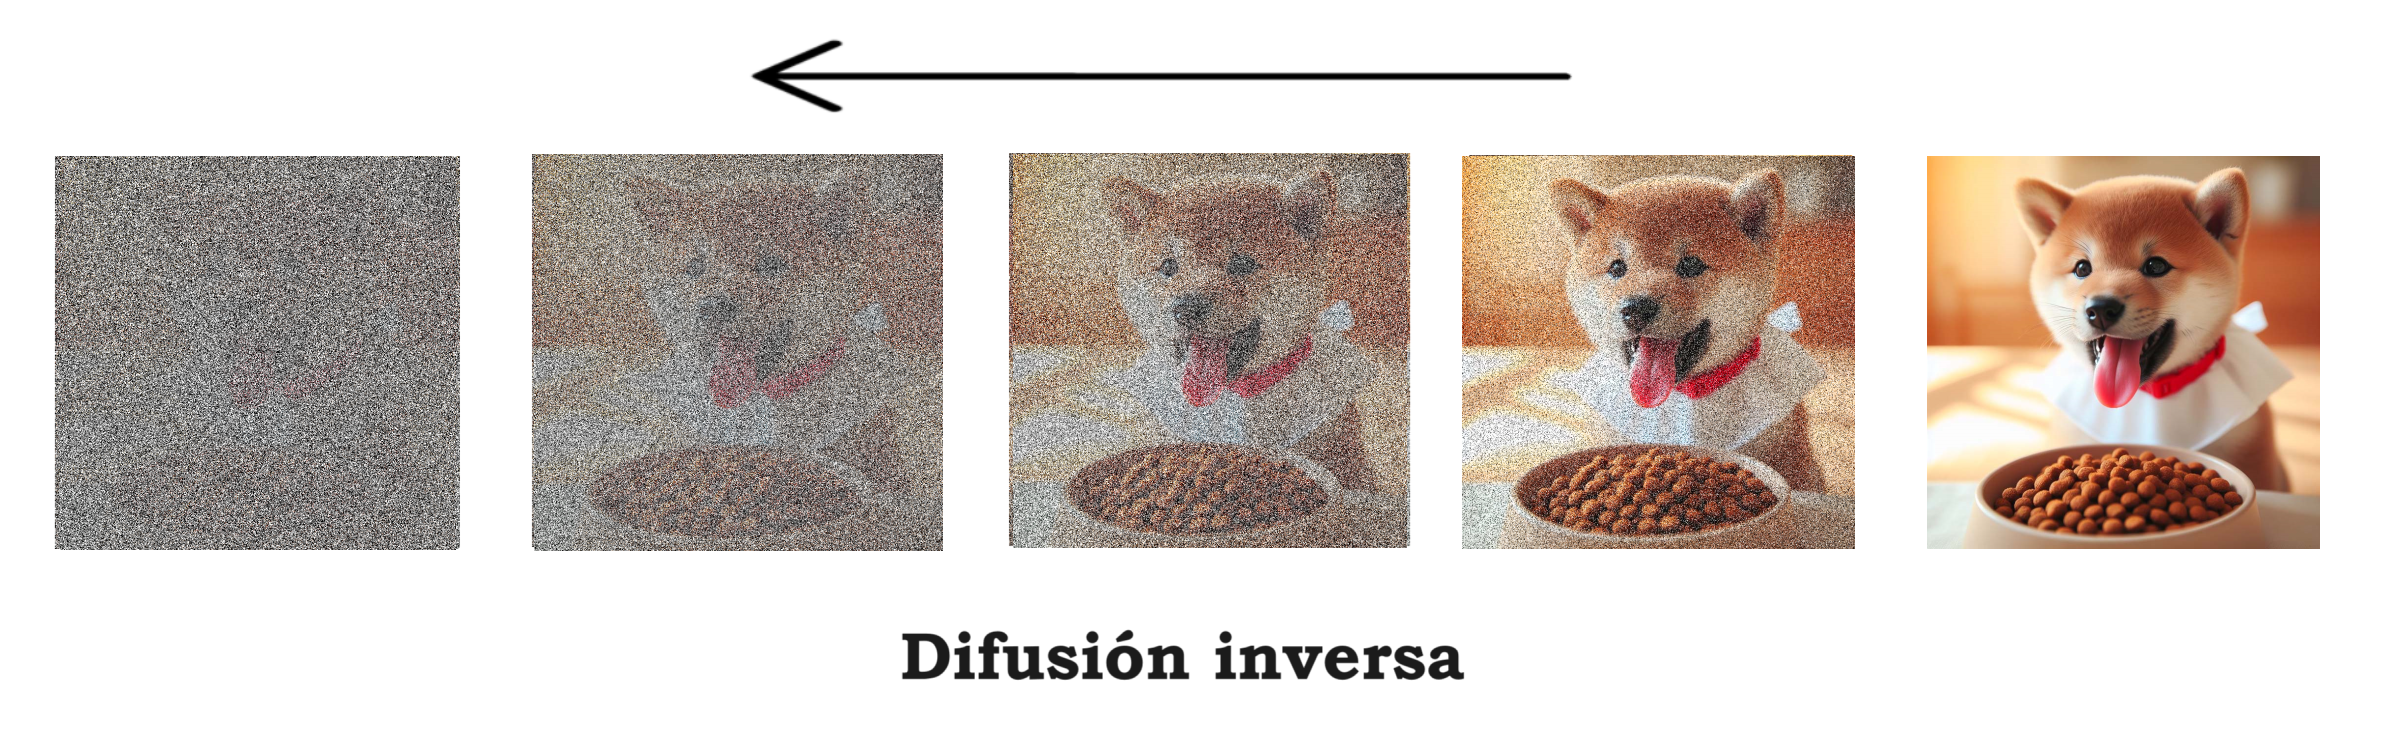
\includegraphics[width = 1 \textwidth]{Imagenes/Vectorial/difusioninversa.png}
	\caption{difusión inversa de una imagen de un cachorro de Shiba Inu comiendo}
	\label{fig:difusioninversa}
\end{figure}

Una vez tenemos la imagen llena de ruido y la forma de calcular el ruido que hay en cada imagen para poder eliminarlo, se empieza el proceso al que llamamos sampler o muestreo. Aquí es cuando entra un componente importante llamado noise scheduler, cuya función es determinar la cantidad de ruido que se debe suprimir en cada paso para alcanzar la forma óptima y que se puedan evitar cambios bruscos entre paso y paso, que sea de forma gradual y que los detalles se vayan puliendo conforme la imagen vaya cobrando más forma. El proceso de muestreo se repite la cantidad de steps o pasos especificada por el usuario. Y de esta manera, concluimos con el primer componente del modelo de difusión latente: la difusión.\\ 

Pasemos a la segunda pieza del puzzle: el espacio latente. El proceso de difusión, por lo que hemos podido ver, es un proceso algo lento y costoso al tener que trabajar con los pixeles de una imagen. Si tenemos una imagen en color con la escala RGB de 512x512 píxeles, estamos hablando de una multiplicación de 3x512x512, es decir, un espacio de casi 80 mil dimensiones. Para solucionar este problema, se trabaja con el espacio latente que trata de reducir la imagen a una escala de 64x64 píxeles, asegurando mayor velocidad y una menor carga de trabajo al trabajar, de esta forma, con unas dimensiones más pequeñas de apenas 12 mil. 

\begin{figure}[h]
	\centering
	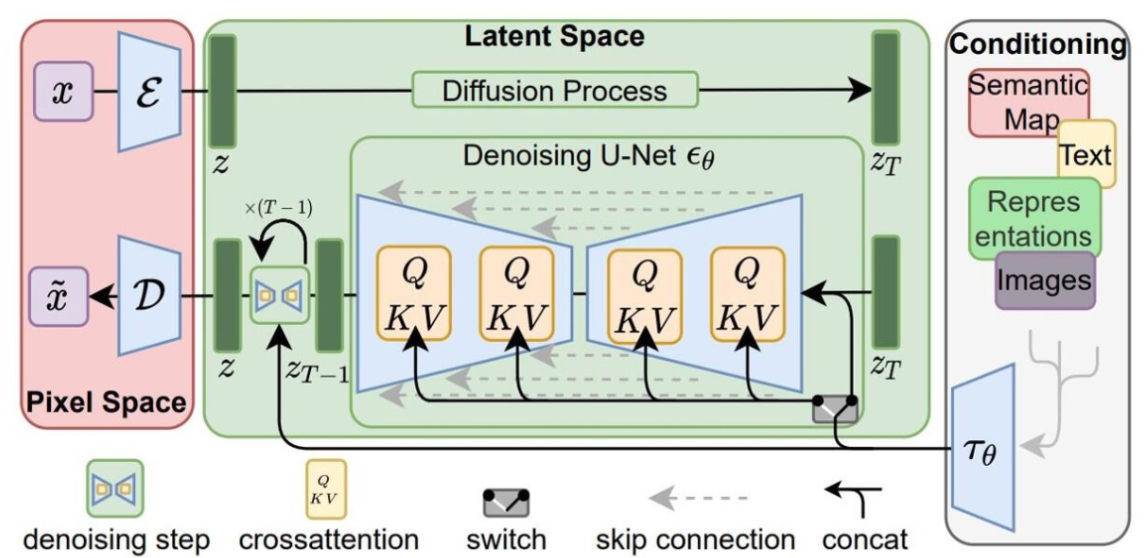
\includegraphics[width = 1
	\textwidth]{Imagenes/Vectorial/espaciolatente.png}
	\caption{Representación gráfica del proceso de conversión al espacio latente}
	\label{fig:latentspace}
\end{figure}

Ahora que entendemos el propósito y el funcionamiento de las dos variables del modelo de difusión latente, profundicemos más en cómo se lleva a cabo cada uno de estos dos procesos y qué mecanismos se utilizan para ello. El modelo se compone principalmente de 3 componentes:\\

Un codificador de texto basado en redes transformer, una red U-Net compuesta de dos redes ResNet y un autocodificador variacional (VAE).\\

\underline{Codificador de texto basado en Transformers}: para producir la imagen que deseamos, previamente es necesario escribir una descripción detallada de la imagen y es por tanto, el primer paso. Este texto que le introducimos al modelo se conoce como prompt y es de lo que se encarga de procesar el codificador de texto.  Lo primero que realiza el text-encoder de Stable Diffusion es a través de un modelo llamado CLIP (Contrastive Language-Image Pre-Training) que se encarga de ofrecer una descripción detallada de las imágenes a través de su propio tokenizador. El siguiente paso y como ya hemos visto en apartados anteriores, el transformer se encarga de realizar la fase de embedding en la que se transforman las palabras de texto en tokens que la red neuronal pueda entender y manejar, para que después, a través del método de self-attention, se decida qué palabras son las que más relevancia tienen.\\ 
 
Además, Stable Diffusion ha añadido a esto una pequeña variación y mejora que añade a esta última técnica, otra llamada cross-attention (o atención cruzada) con la que se permite crear relaciones entre los diferentes embedding y mejorar la precisión del resultado. Por ejemplo, si el prompt pedido es “unas flores pequeñas sobre una bicicleta azul”, solamente con la técnica de self-attention podría procesarse una imagen que fuera “una flor azul sobre una bicicleta pequeña”, lo cual es válido para esa arquitectura pero no es lo que el usuario ha pedido. En cambio, con la ayuda de la técnica de atención cruzada se crean relaciones que tienen más a menos distancia, en la que en este ejemplo la relación flores con azul tiene más distancia que la relación de flores con pequeña, y por tanto, es esta última la que se utilizaría al tener más relación y menos distancia.\\

\underline{Red neuronal U-Net}: es una red neuronal convolucional entrenada para identificar e intentar predecir la cantidad de ruido contenida en una imagen. Consta de un codificador y un decodificador en los que cada uno de estos componentes son, a su vez, bloques ResNet, que son redes convolucionales profundas compuestas por una gran cantidad de capas. La función del codificador se basa en reducir la calidad de la resolución de la imagen mientras que  la función del decodificador es la contraria, generar la imagen en la máxima resolución posible. Entre ambos componentes se añaden conexiones de acceso directo para evitar la pérdida de información importante. Al final, lo que se pretende conseguir es que la red U-Net consiga determinar el ruido para posteriormente, poder conseguir una representación libre de ruido en la imagen final.

\begin{figure}[!htb]
	\centering
	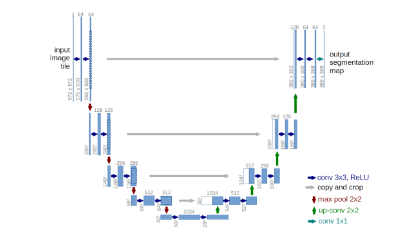
\includegraphics[width = 1
	\textwidth]{Imagenes/Vectorial/u-net.png}
	\caption{Arquitectura de una red U-Net}
	\label{fig:unet}
\end{figure}

\underline{Autocodificador variacional VAE}: es un tipo de red neuronal que al igual que las redes U-Net consta de dos componentes: un codificador y un decodificador, sin embargo sus funciones distan mucho las unas de las otras. El primer componente del autocodificador variacional se encarga de uno de los primeros pasos que realiza Stable Diffusion, que es convertir el espacio de píxeles de la imagen en un tensor dentro del espacio latente de menores dimensiones sustrayendo las características más relevantes de la imagen original y comprimiéndolas en el tensor latente. Y al final del proceso de difusión, se parte del tensor del espacio latente con el que se ha trabajado, para transformarlo en la imagen final generada en una escala de 512x512 píxeles.

\begin{figure}[!hbt]
	\centering
	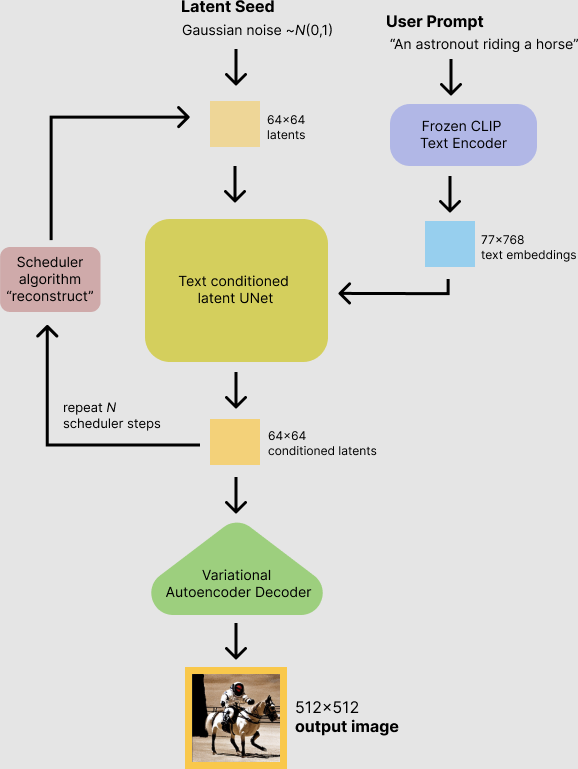
\includegraphics[width = 0.9
	\textwidth]{Imagenes/Vectorial/representacionvisualSD.png}
	\caption{Representación gráfica del funcionamiento de Stable Diffusion}
	\label{fig:sd}
\end{figure}

